\begin{frame}[standout]
  \large\fontspec{xkcd-script.ttf}[Path=./fonts/, Ligatures=TeX]
  ``Your paper makes no goddamn sense, \\
  but it's the most beautiful thing \\
  \XeTeXglyph\XeTeXglyphindex"I_hyphen_p_r_o_n_o_u_n"\relax\
  have ever laid eyes on.''

  \small
  \hfill From r/ProgrammerHumor
  \href{https://www.reddit.com/r/ProgrammerHumor/comments/2jf7yl}{\faRedditAlien}
\end{frame}

\section{介绍}

\begin{frame}{历史回眸}
\begin{columns}
\begin{column}{0.45\textwidth}
  \begin{figure}
    \centering
    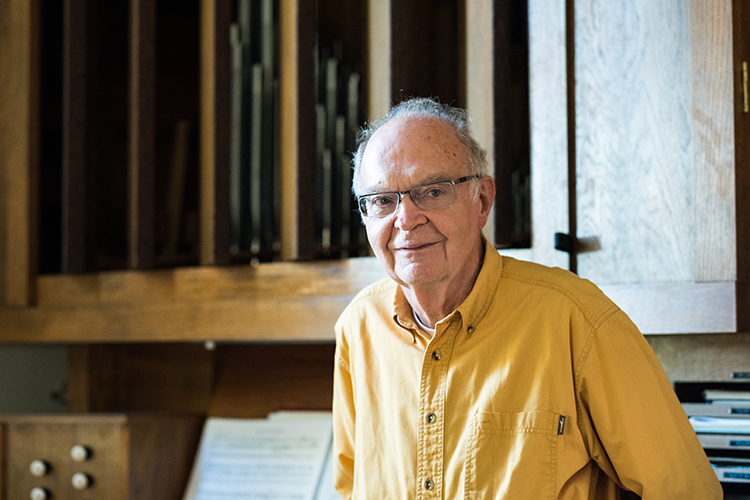
\includegraphics[height=3.2cm]{figures/Knuth-vivian20181019E.jpg}
    \caption{高德纳(Donald~E. Knuth)\footnotemark \\ \TeX}
  \end{figure}
\end{column}
\begin{column}{0.45\textwidth}
  \begin{figure}
    \centering
    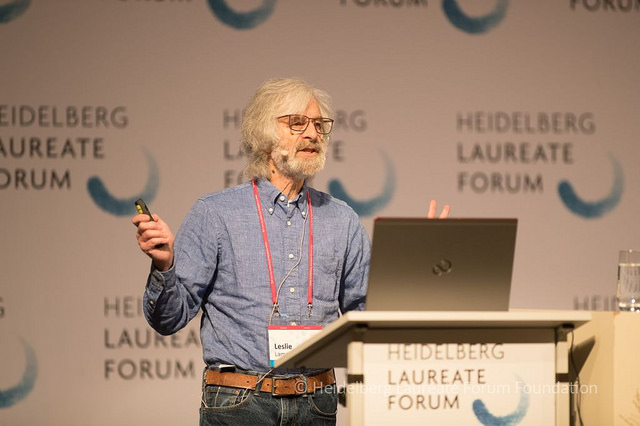
\includegraphics[height=3.2cm]{figures/lamport-2018.jpg}
    \caption{Leslie Lamport~\footnotemark \\ \LaTeX}
  \end{figure}
\end{column}
\end{columns}
\footnotetext[1]{图片来源:\url{https://www-cs-faculty.stanford.edu/~knuth/graphics.html}}
\footnotetext[2]{图片来源:\url{https://aperiodical.com/2018/09/hlf-blogs-leslie-lamport-thinks-your-code-is-bad}}
\end{frame}

\begin{frame}{\LaTeX{} 是什么?}
\begin{itemize}
  \item 打公式方便?
  \item 写论文神器?
  \item 排版语言 + 标记语言 + 宏语言?
\end{itemize}
\end{frame}

\begin{frame}[fragile]
\frametitle{\LaTeX{} 是什么?\mbox{}——\mbox{}What you \emph{think} is what you get!}
\begin{columns}
\begin{column}{0.48\textwidth}
  \begin{texcode}[basicstyle=\tiny\ttfamily, moretexcs={\maketitle},
    emph={[1]equation,itemize,document},emph={[2]article,amsmath,graphicx}]
  \documentclass{article}
  \usepackage{amsmath,graphicx}
  \title{Normal distribution}
  \author{Wikipedia, the free encyclopedia}

  \begin{document}
  \maketitle
  \section{Introduction}
  % 省略一些内容……
  The probability density of the normal
  distribution is
  \begin{equation}
    f(x|\mu, \sigma)
    = \frac{1}{\sqrt{2\pi\sigma^2}}
      e^{-\frac{(x-\mu)^2}{2\sigma^2}}
  \end{equation}
  where
  \begin{itemize}
    \item $\mu$ is the mean of the distribution
    \item $\sigma$ is the standard deviation
  \end{itemize}
  \end{document}
  \end{texcode}
\end{column}
\begin{column}{0.48\textwidth}
  \begin{figure}
    \centering
    \vspace{-0.8cm}
    \includegraphics[width=\textwidth]{example/normal-dist.pdf}
  \end{figure}
\end{column}
\end{columns}
\end{frame}

\begin{frame}{基本原则}
\begin{itemize}
  \item 排版 \textit{vs} 文字处理
    \begin{itemize}
      \item 《别把 \LaTeX{} 当 Word 用》
    \end{itemize}
  \item 遵循业\zhparen{xué}界\zhparen{xiào}规范
    \begin{itemize}
      \item 《管教务处 \textit{or} 研究生院 \textit{or} 物理系叫爸爸》
    \end{itemize}
  \item 追求良好的阅读体验\zhparen{readability}
  \item 内容与格式分离
  \item \alert{内容永远比格式重要!}
\end{itemize}
\end{frame}
